\documentclass[12pt]{book}

\usepackage[dvips,letterpaper,margin=0.75in,bottom=0.5in]{geometry}
\usepackage{cite}
\usepackage{slashed}
\usepackage{graphicx}
\usepackage{amsmath}
\usepackage{braket}
\begin{document}

\newcommand{\ihbar}{\ensuremath{i \hbar}}
\newcommand{\Pss}{\ensuremath{\Psi^*}}
\newcommand{\dPsidt}{\ensuremath{ \frac{\partial \Psi}{\partial t} }}
\newcommand{\dPsidx}{\ensuremath{ \frac{\partial \Psi}{\partial x} }}
\newcommand{\ddPsidx}{\ensuremath{ \frac{\partial^2 \Psi}{\partial x^2} }}
\newcommand{\dPssdt}{\ensuremath{ \frac{\partial \Psi^*}{\partial t} }}
\newcommand{\dPssdx}{\ensuremath{ \frac{\partial \Psi^*}{\partial x} }}
\newcommand{\ddPssdx}{\ensuremath{ \frac{\partial^2 \Psi^*}{\partial x^2} }}

\title{PHY 115A \\ Lecture Notes}
\author{Michael Mulhearn}

\maketitle

\chapter{The Wave Function}

\section{The Experimental Foundation of Quantum Mechanics}

\begin{figure}[thb]
\begin{center}
{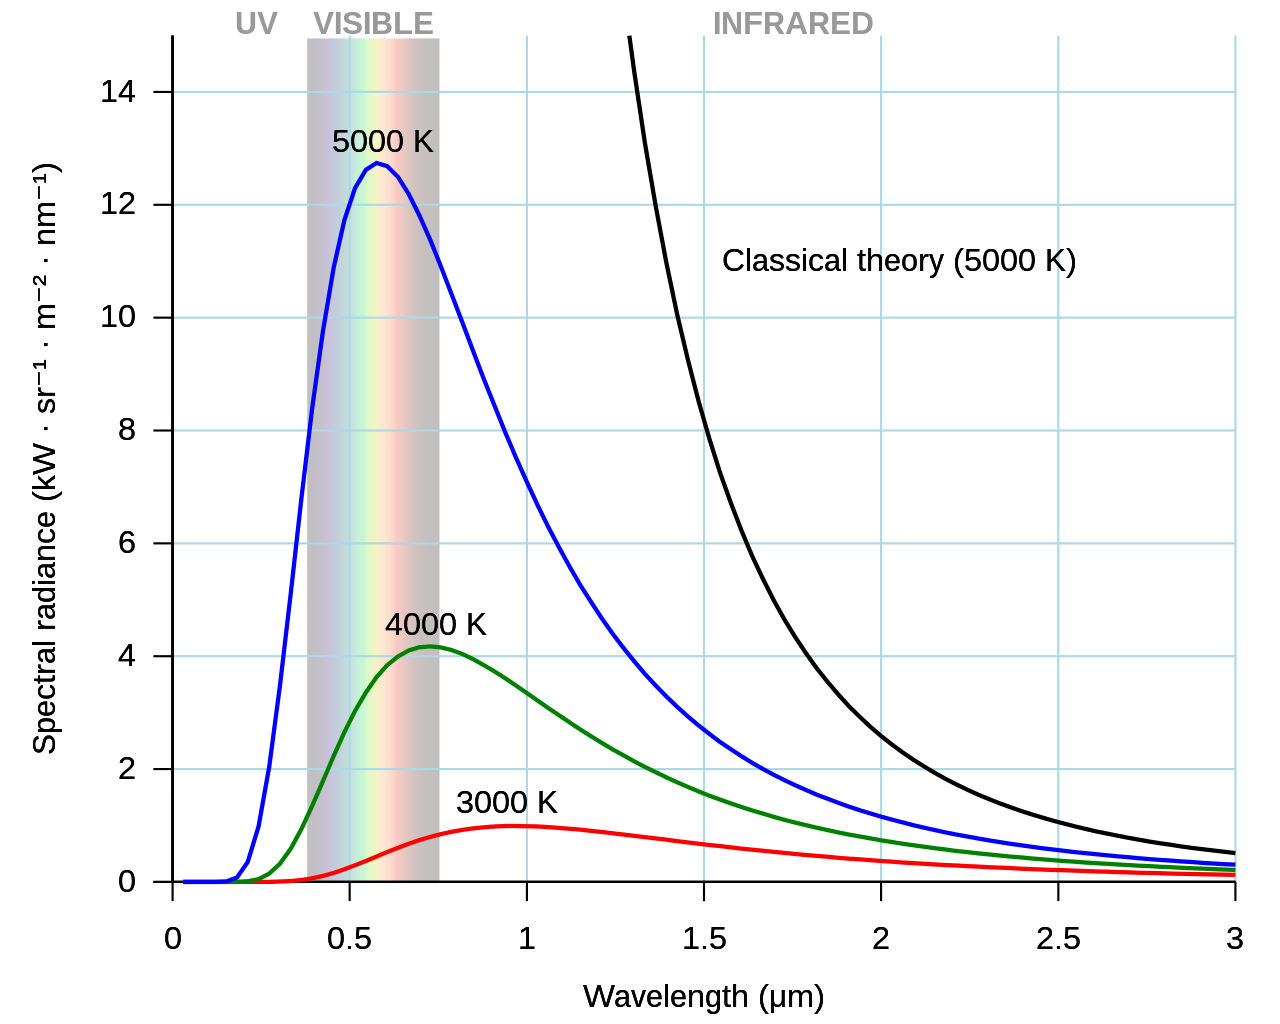
\includegraphics[width=0.40\textwidth]{figs/black_body.png}}
\end{center}
\caption{\label{fig:blackbody} The utraviolet catastrophe.}
\end{figure}

By the start of the 1900's classical physics had achieved a series of remarkable experimental and theoretical breakthroughs.
\begin{itemize}

\item Young's Double Slit experiment (1801) showed that when monochromatic light passes through a single slit followed by two double slits, the intensity of the light reaching a distant plane exhibits an interference pattern:
\begin{displaymath}
I(\theta) = I_0 \, \cos^2\left(\frac{\pi d}{\lambda} \sin \theta \right)
\end{displaymath}
where $\lambda$ is the wavelength of the light, $d$ the distance between the slit, $\theta$ the angle relative to the center of the slits, and $I_0$ the intensity at $\theta=0$.  

\item The Maxwell Equations (1861) unified the magnetic and electrical forces within a theory that accurately describes an array of phenomenon that is breathtaking in scope.  It predicted radio waves and how to produce and detect them.  It alluded to special relativity.  The theory showed that light was a propagating disturbance in the electromagnetic field: an EM wave.
\item JJ Thomson discovered the electron (1897) using cathode ray tubes and determined its charge to mass ratio.  The Millikan oil drop experiment (1909) determined the electron charge $e$.
\end{itemize}
Despite these impressive achievements, their were also shortcomings in the classical theory:
\begin{itemize}
\item The prediction of the classical theory for the spectral radiance of black body radiation failed spectacularly at low wavelength.
\item In the photoelectric effect, light shining on a material causes the emission of electrons.  The classical theory predicts that the kinetic energy of the photoelectrons emitted depends on the intensity of the light, but experiments showed it depended on the wavelength.  Below a certain wavelength for each material, there was no emission at all.
\item Atomic spectroscopy: hydrogen (and other atoms) were shown to emit electromagnetic radiation at specific wavelengths.  For the hydrogen atom, the quantized wavelengths are described by the empirically-determined Rydberg formula:
\begin{displaymath}
\frac{1}{\lambda} = R_H \left( \frac{1}{n_1^2} - \frac{1}{n_2^2} \right)
\end{displaymath}
where $1/R_H = 91~\rm nm$ and $n_1 < n_2$ are both quantum numbers.
\end{itemize}
The explanation for these phenomenon relied upon quantization: 
\begin{itemize}
\item Planck's Law: the observed spectral radiance from black body radiation can be accurately predicted if light consists of discrete quanta, called photons, with energy 
$$E = h \nu.$$  
The ultra-violet catastrophe is avoided because it requires a great deal of energy to produce each ultra-violet photon.   
\item The surprising features of the photoelectric effect can also be understood as do to photons.  Individual photons below a certain wavelength do not have enough energy to liberate an electron, and the kinetic energy of the electrons depends on the energy of the photon, which depends on the wavelength of light, not the intensity. 
\item The Bohr model of the atom constrained electrons to orbits at discrete energy levels with angular momentum that is an integer ratio of Planck's constant.  This model perfectly predicted the Rydberg formula.
\end{itemize}

The quantization of photons inspired Louis de Broglie to the hypothesis that matter behaves like a wave with wavelength
$$ \lambda = \frac{h}{p}.$$
This hypothesis was the beginning of our modern formulation of quantum mechanics.  Modern demonstrations of electron interefernce, as shown in Fig.~\ref{fig:elecint}, clearly reveal the wave nature of matter.

\begin{figure}[thb]
\begin{center}
{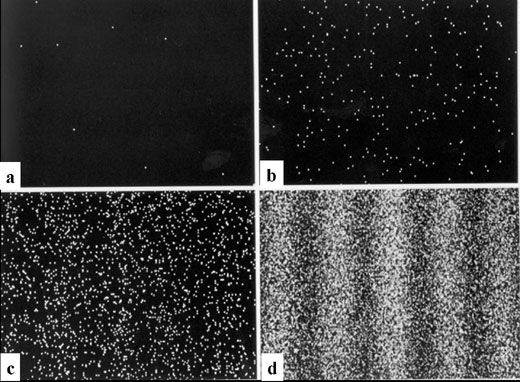
\includegraphics[width=0.40\textwidth]{figs/electron_interference.jpg}}
\end{center}
\caption{\label{fig:elecint} After passing through a double slit apparatus, the location of individual electrons are observed as dots of light.  When enough electrons are observed an interference pattern emerges.}
\end{figure}

The fascinating conversation between theory and experiment that led to the formulation of quantum mechanics is worthy of studying.  However, it isn't the easiest ways to come to terms with the shocking theory.  Instead of developing the theory piece by piece, we'll jump right to the Schr\"odinger Equation as our starting assumption, and work through the consequences.

\section{An Experimental Perspective}

\begin{itemize}

\item Never forget that physics is an {\bf experimental discipline}: the most compelling mathematical argument you can imagine could be rendered invalid by a single well-executed experiment.  

\item {\bf You cannot derive Quantum Mechanics.}  Quantum Mechanics is a set
of assumptions that are mathematically consistent with experimental results.
It offers no explanation for those assumptions.

\item {\bf Derivations are useful for predicting the outcomes of future
experiments} based on the results from our previous experiments, within
the context of a theory.  The more successful we are at playing this little
game, the more confidence we have in the theory.

\item By this metric, {\bf Quantum Mechanics is an exceptionally successful theory!}

\item {\bf The starting assumptions are not unique.} You can learn
a lot by seeing how different assumptions lead to the same physical
theory.  We'll do some of this.

\end{itemize}

\section{The Schr\"odinger Equation}

Here's a summary of Griffiths sections 1.1-1.2.

\begin{itemize}

\item A state of a particle is described by its wave function $\Psi(x,t)$.

\item The wave function $\Psi(x,t)$ is a solution to the Schr\"odinger Equation (SE):
\begin{equation}
\label{eqn:se}
\ihbar \dPsidt = - \frac{\hbar^2}{2 m}\ddPsidx + V \Psi
\end{equation}
where $m$ is the mass of the particle, $V$ the potential energy function or just ``potential'', and:  

\item The reduced plank's constant $\ihbar = \frac{h}{2 \pi} = 1.054573 \times 10^-34~\rm Js$.

\item The physical interpretation of the wave function is statistical.  The probability $P_{ab}(t)$ that the particle will be found between points $a$ and $b$ at time $t$ is:
\begin{equation}
\label{eqn:prob}
P_{ab}(t) = \int_a^b |\Psi(x,t)|^2 dx
\end{equation}
\end{itemize}

Suppose we divide the $x$-axis into six regions $A,B,C,D,E,F$ and the particle is in a state where it has equal probability to be found in any region at $t=0$.  At $t-0$ we observe the particle in region $C$.  Where was the particle before this measurement?  There are several schools of thought:
\begin{itemize}
\item realist:  The particle was already in region $C$ and we just didn't know that yet.
\item orthodox:  The particle wasn't in any one region, it was the measurement itself that caused one of several possible outcomes.
\item agnostic:  I don't know.  It doesn't matter where the particle was before a measurement, because physics is about predicting the outcome of measurements.
\end{itemize}
As we'll see later, John Bell showed that this seemingly philosophical question could be explored experimentally.  Of these three possibilities, the orthodox interpretation is the most supported by the experimental evidence.

\section{Review of Statistics and Probability}

Given that the physical interpretation of Quantum Mechanics is statistical, we'll review the relevant concepts from statistics. This is also covered in Griffiths sections 1.3.  

We refer to the outcome of a random process as a random variable.  Random variables can be discrete (countable): heads or tails from a coin flip, the number of children the next person you meet has had, the number of nuclear decays of a radioactive sample within a specified time interval.  Or random variables can be continuous:  the mass of fish that you have caught, the amount of time you must wait for the next bus to arrive, or the speed of the next bike that passes you.  Here we'll use variable $m$ for a discrete random variables that take on a countable number of distinct values $m=0,1.2,3,\ldots$.  We'll use $x$ to describe a continuous random variable $x$ on the interval $[-\infty, \infty]$. 

\subsection{Discrete and Continuous Random Variables}

In the discrete case, the probability of each outcome $m$ defines the probability distribution function $P(m)$.  To calculate the probability $P_{AB}$ that an outcome $m$ is any integer from $A$ to $B$ we need only sum the probability distribution function for those integers:
\begin{displaymath}
P_{AB} = \sum_{m=A}^{B} P(m).
\end{displaymath}
Because the probability of the outcome being any possible value is 1, we have the normalization condition:
\begin{displaymath}
\sum_{m=0}^{\infty} P(m) = 1
\end{displaymath}

In the case of a continuous random variable $x$, it is nonsensical to speak of the probability of any particular value of $x$.  Instead the probability of $x$ occurring within an interval $a < x < b$:
\begin{displaymath}
P_{ab} = \int_{a}^{b} \rho(x) \, dx
\end{displaymath}
The value of the probability distribution function $\rho(x)$ is not a probability, but instead a probability density, which we integrate to find the probability.  As the outcome must be some value of $x$ between $-\infty$ and $+\infty$ the normalization is:
\begin{displaymath}
\int_{-\infty}^{+\infty} \rho(x) \, dx = 1
\end{displaymath}
The probability distribution function of a continuous random variable is called a probability density function (PDF).  A discrete probability distribution is sometimes referred to
as probability mass function (PMF), to draw upon an analogy with physical mass and density: a PDF is probability per unit volume (1-D volume in this case) while
a PMF is simply a probability.

\subsection{Mean and Variance}

Given a probability distribution our most urgent questions are generally ``what is a
typical outcome?'' and ``how widely will outcomes typically vary from
one another?''.  There are a number of ways to give a quantitative answer to the first question,
but generally the most useful answer is the mean value of the
distribution, $\mu$, which we calculate as a weighted average across
all possible outcomes.  For a discrete random variable we calculate a sum:
\begin{equation}
\label{eqn:mudis}
\mu = \sum_{m=0}^{\infty} m \, P(m)
\end{equation}
For a continuous probability distribution we integrate instead:
\begin{equation}
\mu = \int_{-\infty}^{+\infty} x \, \rho(x) \, dx 
\end{equation}
across a range appropriate to the situation, typically $[-\infty,\infty]$.

The mean value is an example of an expectation value.  In general, the
expectation value of a function $f(x)$ of a random variable $x$ drawn
from a probability distribution function $P(x)$ is:
\begin{displaymath}
\braket{f(x)} \equiv \int_{-\infty}^{+\infty} f(x) \, \rho(x) \,dx.
\end{displaymath}
For a discrete random variable, the integral becomes a sum:
\begin{displaymath}
\braket{f(m)} \equiv \sum_m f(m) \, P(m) 
\end{displaymath}
Using this notation, we can define the mean as the expectation value of the random variable:
\begin{displaymath}
\mu \equiv \braket{x}
\end{displaymath}

To answer the second question, we define an expectation value
which characterizes the variation of outcomes from the mean value,
which we call the variance ($\sigma^2$) of the distribution:
\begin{displaymath}
\sigma^2 \equiv \braket{(x-\mu)^2}.
\end{displaymath}
The square root of the variance is referred to as the
standard deviation ($\sigma$).

There are other ways to quantify the variation from outcome to
outcome, but they are generally inferior to the variance in some way.
For example $\braket{x-\mu}$ can be zero, even for wide distributions,
as long as $P(x)$ is symmetric.  The quantity $\braket{|x-\mu|}$
(called the average deviation) avoids this pitfall but is generally
much harder to calculate, due to the absolute value.

The variance, on the other hand, is quite convenient to calculate.
For example, you can show that:
\begin{equation}
\label{eqn:varhw}
\braket{(x-\mu)^2} = \braket{x^2} -\braket{x}^2.
\end{equation}
We need only calculate $\braket{x}$ and $\braket{x^2}$ in order
to determine both the mean and variance of a distribution.

\section{Normalization of the Wave Function}

This material is covered in Griffiths section 1.4.  
\begin{itemize}
 \item If $\Psi(x,t)$ is a solution to the SE, then so is $k \cdot \Psi(x,t)$ for any value $k$ (check!)  So it would seem we could make the probability density $|\Psi(x,t)|^2$ any value that we like and still satisfy the SE!  
 \item In fact, we are constrained in our choice by the realization that the probability of finding the particle {\em somewhere} must be 1, and so we must choose the normalization of $\Psi$ such that:
\begin{equation}
\label{eqn:norm}
\int_{-\infty}^{+\infty} |\Psi(x,t)|^2 dx = 1
\end{equation}

\item If $\Psi(x,t)=0$ for all $x$ we cannot normalize $\Psi$.
 \item If the integral:
$$\int_{-\infty}^{+\infty} |\Psi(x,t)|^2 dx$$
diverges then we cannot normalize $\Psi$.
\item Being good physicists, we simply throw away useless unphysical solutions that cannot be normalized, and we are never troubled by them again! 
\end{itemize}

But now here's a troubling throught.  Suppose at $t=0$, we have normalized $\Psi(x,t)$ such that
$$\int_{-\infty}^{+\infty} |\Psi(x,0)|^2 dx = 1$$.  
From this point on, the time dependence of $\Psi(x,t)$ is given by the SE, outside of our control.  What if changes in such a way that:
$$\int_{-\infty}^{+\infty} |\Psi(x,t)|^2 dx \neq 1$$ 
at later times?  Might we have to renormalize $\Psi(x,t)$ again at each $t$?  What would we make of $d\Psi/dt$ in this case?

Fortunately, solutions to the SE preserve their normalization.  We can show this using the SE and integration by parts (reviewed above).  We note that:
$$\frac{d}{dt}\int_{-\infty}^{+\infty} |\Psi(x,t)|^2 \, dx  = 
\int_{-\infty}^{+\infty} \frac{\partial}{\partial t} |\Psi(x,t)|^2\, dx.$$ 
Working on the integral:
\begin{eqnarray*}
\frac{\partial}{\partial t} |\Psi(x,t)|^2 &=&  \frac{\partial}{\partial t} (\Psi^* \Psi) \\[7pt]
  &=&  \frac{\partial \Psi^*}{\partial t} \Psi + \Psi^* \frac{\partial \Psi}{\partial t} \\
\end{eqnarray*}
Reworking SE:
\begin{eqnarray*}
\label{eqn:se}
\ihbar \dPsidt &=& -  \frac{\hbar^2}{2 m}\,\ddPsidx + V \Psi \\[7pt] 
       \dPsidt &=& \;\; \frac{\ihbar}{2 m}\,\ddPsidx - \frac{i V}{\hbar} \Psi \\[7pt]
       \dPssdt &=& - \frac{\ihbar}{2 m}\,\ddPssdx + \frac{i V}{\hbar} \Psi^* \\[7pt]
\end{eqnarray*}
where in the last step we've taken the complex conjugate of the preceding equation.  Substituting these results we have:
\begin{eqnarray}
\frac{\partial}{\partial t} |\Psi(x,t)|^2 &=&  \frac{\ihbar}{2 m} 
\left( \Psi^* \ddPsidx - \ddPssdx \Psi\right) \notag \\[7pt]
\label{eqn:dtpp}
  &=& \frac{\ihbar}{2 m} \;
\frac{\partial}{\partial x} \, \left( \Psi^* \dPsidx - \dPssdx \Psi\right)
\end{eqnarray}
So now:
\begin{eqnarray*}
\frac{d}{dt}\int_{-\infty}^{+\infty} |\Psi(x,t)|^2 \, dx  &=& 
\frac{\ihbar}{2 m} \, \int_{-\infty}^{+\infty}  \frac{\partial}{\partial x} \, \left( \Psi^* \dPsidx - \dPssdx \Psi\right) dx\\[7pt]
&=&  \frac{\ihbar}{2 m} \, \left. \left( \Psi^* \dPsidx - \dPssdx \Psi\right) 
\right\rvert_{-\infty}^{+\infty}\\[7pt]
&=& 0
\end{eqnarray*}
where in the last step we've used the fact that the wave function and it's derivative must go to zero at infinity to be physical.

\section{Review of Integration by Parts}

We'll make use of integration by parts in the following sections, so let's review the idea.  We apply the chain rule to the functions $u(x)$ and $v(x)$:
$$\frac{d(uv)}{dx} = u\frac{dv}{dx} + v\frac{du}{dx}$$
and then integrate both sides:
$$\int_a^b\frac{d(uv)}{dx} \, dx = \int_a^b u \frac{dv}{dx} \, dx + \int_a^bv\frac{du}{dx} \, dx$$
By the fundamental theorem of calculus:
$$\int_a^b\frac{d(uv)}{dx} = \left. uv \right\rvert_{a}^{b}$$
If the product $u(x)\,v(x)$ vanishes at $x = a$ and $x = b$ then
$$\left.uv \right\rvert_{a}^{b} = 0$$
and so:
\begin{equation}
\label{eqn:intparts}
\int_{a}^{b} u \frac{dv}{dx} \, dx =  - \int_{a}^{b} v \frac{du}{dx} \, dx
\end{equation}
Suppose a definite integral consists of two parts, one of which ($dv/dx$ here) is a derivative with respect to the integration variable ($x$ here).  Further suppose that the integrand with the derivative removed ($uv$ here) vanishes at the limits of the integration.  In this case, we can move the differentiation between parts of the integrand (from $v$ to $u$ here) by adding a negative sign.

\section{Position and Momentum Operators}
\begin{itemize}
\item  From the probability interpretation of the wave function $\rho(x) = | \Psi | ^2$, we define the expectation value of the $x$ position as:
$$\braket{x} \equiv \int_{-\infty}^{+\infty} x \, \rho(x) \,dx = \int_{-\infty}^{+\infty} x \, |\Psi|^2 \,dx$$
\item There is some subtlety here: the expectation value for the observable $x$ is the mean value of the results of many repeated measurements of the $x$ position of a particle {\em always starting} in the same state $\Psi$.  
\item Due to the collapse of the wave function, repeated measurements of the $x$ position of the same particle {\em after} it was already observed at some position $x=a$ would reproduce the same result (to within the experiments ability to do so before the particle's state changes).
\end{itemize}

In classical physics, the state of a particle is completely determined from it's position and momentum.  So it is natural to consider the expectation value for the momentum: 
\begin{eqnarray*}
\braket{p} &=& m \frac{d}{dt} \braket{x} \\[7pt] 
&=& m \int_{-\infty}^{+\infty} x \, \frac{\partial}{\partial t} |\Psi|^2 \,dx \\[7pt]
\end{eqnarray*}
We already worked out the time derivative in the integrand before (Equation~\ref{eqn:dtpp}) so we have:
\begin{eqnarray*}
\braket{p} &=&  \frac{\ihbar}{2} \int_{-\infty}^{+\infty} x \, \frac{\partial}{\partial x} \, \left( \Psi^* \dPsidx - \dPssdx \Psi\right) \,dx \\[7pt]
\end{eqnarray*}
We can use integration by parts to move the outer partial derivative onto the $x$:
\begin{eqnarray*}
\braket{p} &=&  -\frac{\ihbar}{2} \int_{-\infty}^{+\infty} \frac{\partial x}{\partial x} \, \left( \Psi^* \dPsidx - \dPssdx \Psi\right) \,dx \\[7pt]
&=&  -\frac{\ihbar}{2} \int_{-\infty}^{+\infty} \, \left( \Psi^* \dPsidx - \dPssdx \Psi\right) \,dx \\[7pt]
\end{eqnarray*}
And one more application of integration by parts to second term in the parenthesis:
\begin{eqnarray}
\braket{p} &=&  -\ihbar \, \int_{-\infty}^{+\infty} \, \left( \Psi^* \dPsidx \right) \,dx \notag \\[7pt]
 &=& \int_{-\infty}^{+\infty} \, \Psi^* \left[ -\ihbar \frac{\partial}{\partial x}\right] \Psi \,dx 
\label{eqn:derivpop} \end{eqnarray}
Compare to the expectation value for the position:
\begin{eqnarray}
\braket{x} 
 &=& \int_{-\infty}^{+\infty} \, \Psi^* \left[ x \right] \Psi \,dx 
\end{eqnarray}

In general, we calculate expectation value of an observable $o$
using the corresponding {\em operator} $\hat{o}$:
\begin{eqnarray}
\braket{o}  &=& \int_{-\infty}^{+\infty} \, \Psi^* \left[ \hat{o} \right] \Psi \,dx 
\end{eqnarray}
For the position observable we have the position operator 
\begin{equation}
\hat{x} = x.
\end{equation}
For the momentum observable with have the momentum operator 
\begin{equation}
\hat{p} = - \ihbar \frac{\partial}{\partial x}.
\end{equation}
We can construct the operator $\hat{f}$ for any classical function of position and momentum $f(x,p)$ by substituting $\hat{p}$ and $\hat{x}$ for $p$ and $x$.
\begin{eqnarray}
\braket{f(x,p)}  &=& \int_{-\infty}^{+\infty} \, \Psi^* \left[ f(\hat{x},\hat{p}) \right] \Psi \,dx 
\end{eqnarray}
Since the position and momentum completely define the state of a classical particle, any dynamical variable can be calculated from x and p.  Therefore, this is a prescription for calculating the expectation value of any classical dynamical variable.

Have a close look at Equation~\ref{eqn:derivpop}.  Had we applied integration by parts to the first term instead of the section, we would have instead concluded:
\begin{eqnarray*}
\braket{p} &=&  
\int_{-\infty}^{+\infty} \, \left(\left[ \ihbar \frac{\partial}{\partial x}\right] \Psi^* \right) \Psi\,dx 
\end{eqnarray*}
evidently, there is also a momentum operator that operates on the $\Psi^*$.  We'll return to this later.

\section{Ehrenfest's Theorem}
\begin{eqnarray*}
\frac{d \braket{p}}{dt} &=& \frac{d}{dt} \int_{-\infty}^{+\infty} \, \Psi^* \, \hat{p} \, \Psi \,dx \\[7pt]
&=& -\ihbar \int_{-\infty}^{+\infty} \, \frac{\partial}{\partial t} \left(\Psi^* \dPsidx\right) \,dx \\[7pt]
&=& -\ihbar \int_{-\infty}^{+\infty} \, \left( \dPssdt \dPsidx + 
\Psi^* \frac{\partial}{\partial x} \dPsidt \right) \,dx \\[7pt]
\end{eqnarray*}
where in the last part we have used:
$$\frac{\partial}{\partial t} \dPsidx = \frac{\partial}{\partial x} \dPsidt$$
now using integration by parts on the second term:
\begin{eqnarray*}
\frac{d \braket{p}}{dt} &=& -\ihbar \int_{-\infty}^{+\infty} \, 
\left( \dPssdt \dPsidx - \dPssdx \dPsidt \right) \,dx \\[7pt]
&=& -\ihbar \int_{-\infty}^{+\infty} \, 
\left( \left[ -\frac{\ihbar}{2 m}\,\ddPssdx + \frac{i V}{\hbar} \Pss \right] \dPsidx 
- \dPssdx \left[ \frac{\ihbar}{2 m}\,\ddPsidx - \frac{i V}{\hbar} \Psi \right] \right) \,dx \\[7pt]
&=& -\frac{\hbar^2}{2 m} \int_{-\infty}^{+\infty} \, \left(\ddPssdx \dPsidx + \dPssdx \ddPsidx\right)
+ \int_{-\infty}^{+\infty} V \left( \Pss \dPsidx + \dPssdx \Psi \right) \, dx \\[7pt]
&=& -\frac{\hbar^2}{2 m} \int_{-\infty}^{+\infty} \, \frac{\partial}{\partial x} \left(\dPssdx \dPsidx + \dPssdx \dPsidx\right) dx
+ \int_{-\infty}^{+\infty} V \frac{\partial}{\partial x} \left( \Pss \Psi \right) \, dx \\[7pt]
\end{eqnarray*}
The first integral vanishes\footnote{If you want to go for the hat trick (three scores in one game) on using integration by parts, you can do it here, noting that $d1/dx = 0$.} and using integration by parts on the second integrand:
\begin{eqnarray*}
\frac{d \braket{p}}{dt} &=& -\int_{-\infty}^{+\infty} \frac{\partial V}{\partial x} \Pss \Psi \, dx \\[7pt]
\end{eqnarray*}
so now:
\begin{eqnarray}
\label{eqn:ehrenfest}
\frac{d \braket{p}}{dt} &=& - \braket{\frac{\partial V}{\partial x}}
\end{eqnarray}
which is known as Ehrenfest's Theorem.

Newton's Law in one dimension in classical physics can be written as:
\begin{eqnarray}
\label{eqn:ehrenfest}
\frac{dp}{dt} &=& -\frac{dV}{dx}
\end{eqnarray}

which remains true in Quantum Mechanics in an average sense.

\section{The Uncertainty Principle}

From our review of statistics we know that the variance of $x$ can be calculated as:
\begin{displaymath}
\sigma_x^2 \equiv \braket{\,(x-\braket{x})^2\,} = \braket{x^2}-\braket{x}^2
\end{displaymath}
where:
\begin{eqnarray}
\braket{x} 
 &=& \int_{-\infty}^{+\infty} \, \Psi^* \left[ \hat{x} \right] \Psi \,dx \\
 &=& \int_{-\infty}^{+\infty} \, x|\Psi|^2 \,dx 
\end{eqnarray}
and
\begin{eqnarray}
\braket{x^2} 
 &=& \int_{-\infty}^{+\infty} \, \Psi^* \left[ \hat{x}^2 \right] \Psi \,dx \\
 &=& \int_{-\infty}^{+\infty} \, x^2|\Psi|^2 \,dx 
\end{eqnarray}

The variance of $p$ is:

\begin{displaymath}
\sigma_p^2 \equiv \braket{\,(p-\braket{p})^2\,} = \braket{p^2}-\braket{p}^2
\end{displaymath}
where:
\begin{eqnarray}
\braket{x} 
 &=& \int_{-\infty}^{+\infty} \, \Psi^* \left[ \hat{p} \right] \Psi \,dx \\[8pt]
 &=& -\ihbar \int_{-\infty}^{+\infty} \, \Psi^* \; \dPsidx \; dx \\
\end{eqnarray}
and
\begin{eqnarray}
\braket{x^2} 
 &=& \int_{-\infty}^{+\infty} \, \Psi^* \left[ \hat{p}^2 \right] \Psi \,dx \\[8pt]
 &=& -\hbar^2 \int_{-\infty}^{+\infty} \, \Psi^* \; \ddPsidx \; dx \\
\end{eqnarray}

The Heisenberg uncertainty principle states that:
\begin{equation}
\sigma_x \sigma_p \, \geq \, \frac{\hbar}{2}
\end{equation}

This is easily the most famous result of quantum mechanics.  But we aren't ready to prove it yet. We will come back to that once we are better equipped to do so.

Griffiths section 1.6 gives a good intuitive explanation that goes like this:
\begin{itemize}
\item The de Broglie hypothesis relates a particles momentum to it's wavelength:
\begin{equation}
p = \frac{h}{\lambda}
\end{equation}
(we aren't equipped yet to proof this yet either)
\item Waves that have a well defined wavelength (e.g. an entire sine wave) do not have a well defined position.
\item Waves that have a well defined position (e.g. a localized splash) do not have a well defined wavelength.
\end{itemize}

Don't worry if this doesn't seem clear yet.  We'll but this on very firm ground later!

\section{Chapter Review}

We are considering a particle of mass $m$, in one dimension $x$, in a potential $V$.

\begin{itemize}
\item The state of a particle is described by its wave function $\Psi(x,t)$.
\item The wave function $\Psi(x,t)$ is a solution to the Schr\"odinger Equation (SE):
\begin{equation}
\label{eqn:se}
\ihbar \dPsidt = - \frac{\hbar^2}{2 m}\ddPsidx + V \Psi
\end{equation}
\item The physical interpretation of the wave function is statistical.  The probability $P_{ab}(t)$ that the particle will be found between points $a$ and $b$ at time $t$ is:
\begin{equation}
\label{eqn:prob}
P_{ab}(t) = \int_a^b |\Psi(x,t)|^2 dx
\end{equation}
\item The wave functions are normalized such that
\begin{equation}
\int_{-\infty}^{+\infty} |\Psi(x,t)|^2 dx = 1
\end{equation}
\item Once a wave function is normalized, it will remain normalized for all time as a consequence of the Schr\"odinger equation.
\item Measurements of observable quantities are associated with operators.  Given an operator $\hat{o}$ we can calculate the expectation value for the observable $o$ as:
\begin{eqnarray}
\braket{o}  &=& \int_{-\infty}^{+\infty} \, \Psi^* \left[ \hat{o} \right] \Psi \,dx 
\end{eqnarray}
The operator acts toward its right.
\item For the position observable with have the position operator 
\begin{equation}
\hat{x} = x.
\end{equation}
\item For the momentum observable with have the momentum operator 
\begin{equation}
\hat{p} = - \ihbar \frac{\partial}{\partial x}.
\end{equation}
\item Any classical dynamical variable can be calculated from the position and momentum, and we can calculate its expectation value as:
\begin{eqnarray}
\braket{f(x,p)}  &=& \int_{-\infty}^{+\infty} \, \Psi^* \left[ f(\hat{x},\hat{p}) \right] \Psi \,dx 
\end{eqnarray}

\item Newtons law is still true, but only in an average sense, by Ehrenfest's Theorem:
\begin{eqnarray}
\frac{d \braket{p}}{dt} &=& - \braket{\frac{\partial V}{\partial x}}
\end{eqnarray}
\item The Heisenberg uncertainty relation states that:
\begin{equation}
\sigma_x \sigma_p \, \geq \, \frac{\hbar}{2}
\end{equation}

\end{itemize}



\end{document}

\chapter{Time-Independent Schr\"odinger Equation}


\chapter{Formalism}





\appendix

\chapter{Fourier Transforms}

\section{The Vector Analogy}

A vector in ordinary space is completely specified by its displacement in each spatial direction.  Lets look at this familiar picture a bit formally, to prepare us to apply it in a less intuitive (but mathematically equivalent) setting.  The first thing we will need to know how to do is to calculate the dot product between any two vectors:  
\begin{displaymath}
\vec{v} \cdot \vec{w} = v_x w_x + v_y w_y + v_z w_z 
\end{displaymath}
You already know how to do this for ordinary vectors.  In other settings, we use the more general term {\em inner product}.  To describe any vector we need a set of {\em basis vectors}, in this case $\hat{x}$, $\hat{y}$, and $\hat{z}$.  These basis vectors are orthogonal:
\begin{displaymath}
\hat{x} \cdot \hat{y} = \hat{y} \cdot \hat{z} = \hat{z} \cdot \hat{x} = 0
\end{displaymath}
and normalized:
\begin{displaymath}
\hat{x} \cdot \hat{x} = \hat{y} \cdot \hat{y} = \hat{z} \cdot \hat{z} = 1.
\end{displaymath}
When the basis vectors have both of these properties, we call them {\em orthonormal}.

For any possible vector $\vec{v}$, we can calculate its component in the direction of each basis vector by calculating the inner product:
\begin{eqnarray*}
v_x = \vec{v} \cdot \hat{x} \\
v_y = \vec{v} \cdot \hat{y} \\
v_z = \vec{v} \cdot \hat{z} \\
\end{eqnarray*}
We say that the basis vectors $\hat{x}$, $\hat{y}$, and $\hat{z}$ are "complete", because specifying the values of $v_x$, $v_y$, and $v_z$ completely describes the vector $v$.  The set of basis vectors $\hat{x}$ and $\hat{z}$ are orthonormal, but they are not complete in three dimensional space, because there are vectors which we cannot write using only these two directions.  For instance, there are no possible values for $v_x$ and $v_z$
which make
\begin{eqnarray*}
 \vec{v_1} = v_x \hat{x} + v_z \hat{z}
\end{eqnarray*}
equal to the vector
\begin{eqnarray*}
 \vec{v_2} = 3 \hat{x} + 2 \hat{y} + 7 \hat{z}.
\end{eqnarray*}

 
\section{The Fourier Series}

Using the language of vectors, the Fourier Theorem states that the sines and cosines form a complete orthonormal basis for describing any periodic function.  

To make sense of this, we need to define the inner product. If we restrict ourselves to real functions of $x$ with period $L$, the inner product between any two functions $f(x)$ and $g(x)$ is defined to be the integral:
\begin{equation}
\braket{f, g} \equiv \int_{-\frac{L}{2}}^{\frac{L}{2}} f(x) g(x) \, dx
\end{equation}
The orthonormal basis vectors are the specific sine and cosine functions
\begin{eqnarray}
s_n(x) \equiv \sqrt{\frac{2}{L}}\sin\left(\frac{2\pi n}{L} \, x \right)\\
c_n(x) \equiv \sqrt{\frac{2}{L}}\cos\left(\frac{2\pi n}{L} \, x \right)
\end{eqnarray}
which are defined for
\begin{eqnarray}
n = 0,1,2,3,...
\end{eqnarray}
These are normalized because by our definition for the inner product we can see that:
\begin{eqnarray*}
\braket{s_n, s_n} &=& \frac{2}{L} \int_{-\frac{L}{2}}^{\frac{L}{2}} \sin^2\left(\frac{2\pi n}{L} \, x \right) \, dx = 1 \\
\braket{c_n, c_n} &=& \frac{2}{L} \int_{-\frac{L}{2}}^{\frac{L}{2}} \sin^2\left(\frac{2\pi n}{L} \, x \right) \, dx = 1
\end{eqnarray*}
The demonstration that they are orthogonal is left as an exercise (See HW Problem 1):
\begin{eqnarray*}
\braket{s_n, s_m} &=& \frac{2}{L} \int_{-\frac{L}{2}}^{\frac{L}{2}} 
\sin\left(\frac{2\pi n}{L} \, x \right) \sin\left(\frac{2\pi m}{L} \, x \right) \, dx = 0 ~~(n \neq m) \\
\braket{c_n, c_m} &=& \frac{2}{L} \int_{-\frac{L}{2}}^{\frac{L}{2}} 
\cos\left(\frac{2\pi n}{L} \, x \right) \cos\left(\frac{2\pi m}{L} \, x \right) \, dx = 0~~(n \neq m) \\
\braket{s_n, c_m} &=& \frac{2}{L} \int_{-\frac{L}{2}}^{\frac{L}{2}} 
\sin\left(\frac{2\pi n}{L} \, x \right) \cos\left(\frac{2\pi m}{L} \, x \right) \, dx = 0 
\end{eqnarray*}
We can combine the normalization and orthogonality conditions using the Kronecker delta symbol:
\begin{displaymath}
\delta_{nm} =  
\left\{
	\begin{array}{ll}
		1  & \mbox{if } n=m \\
		0 & \mbox{otherwise}
	\end{array}
\right.
\end{displaymath}
and write the above five equations as:
\begin{eqnarray}
\braket{s_n, s_m} &=& \frac{2}{L} \int_{-\frac{L}{2}}^{\frac{L}{2}} 
\sin\left(\frac{2\pi n}{L} \, x \right) \sin\left(\frac{2\pi m}{L} \, x \right) \, dx = \delta_{nm} \label{eqn:oss}\\
\braket{c_n, c_m} &=& \frac{2}{L} \int_{-\frac{L}{2}}^{\frac{L}{2}} 
\cos\left(\frac{2\pi n}{L} \, x \right) \cos\left(\frac{2\pi m}{L} \, x \right) \, dx = \delta_{nm} \label{eqn:occ}\\
\braket{s_n, c_m} &=& \frac{2}{L} \int_{-\frac{L}{2}}^{\frac{L}{2}} 
\sin\left(\frac{2\pi n}{L} \, x \right) \cos\left(\frac{2\pi m}{L} \, x \right) \, dx = 0 \label{eqn:osc}
\end{eqnarray}







Last of all, they are {\em complete} because {any periodic function} with period $L$ can be written as a sum of these sines and cosines:
\begin{eqnarray}
f(x) = \sqrt{\frac{2}{L}} \sum_{n=0}^{\infty}  A_n \, \cos\left(\frac{2\pi n}{L} \, x \right) + \sqrt{\frac{2}{L}} \sum_{n=1}^{\infty} B_n \, \sin\left(\frac{2\pi n}{L} \, x \right) \label{eqn:lfs}
\end{eqnarray}
The values $A_n$ and $B_n$ are called {\em Fourier coefficients}.  Technically the $N$th term in the Fourier Series refers to the approximation for $f(x)$ from the first $N$ terms in the infinite sum above, and we say that the Fourier Series converges to the function $f(x)$.  Note that $s_0(x) = 0$, which is why the second sum begins at $n=1$.  The demonstration of completeness is optional reading, available in the Appendix.

For a visual example of the Fourier Series, the first terms of the Fourier Series for a step function are shown in Fig.~\ref{fig:fall}.  

\section{Determining the Fourier Coefficients}
\label{sect:coeff}

\begin{figure}[thb]
\begin{center}
{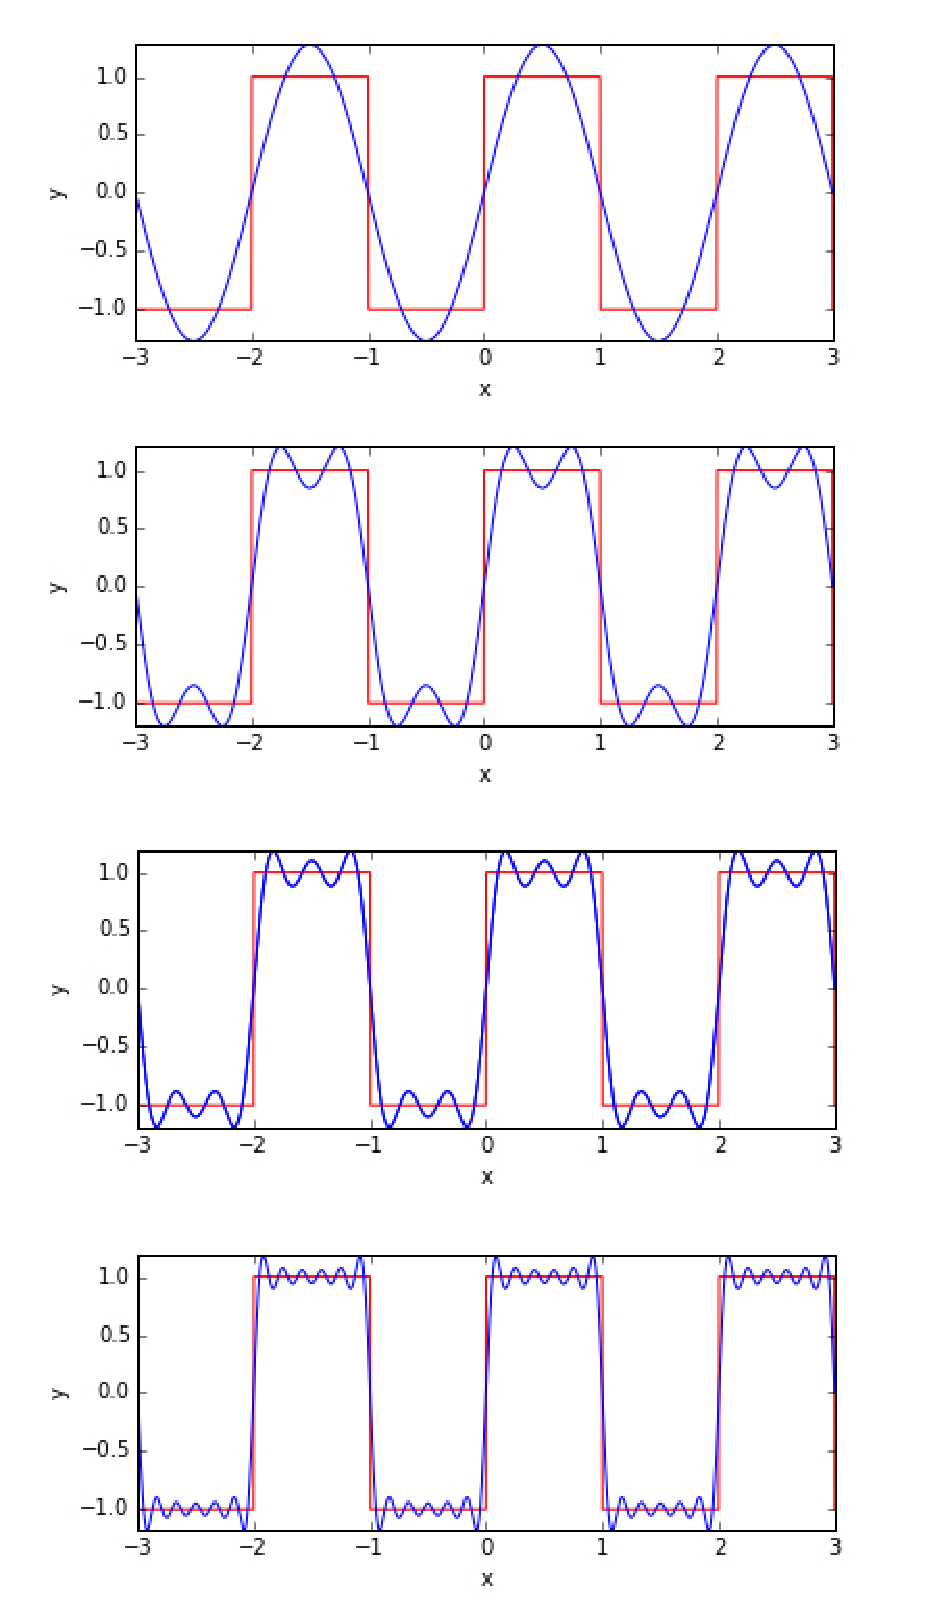
\includegraphics[width=0.40\textwidth]{figs/fsall.pdf}}
\end{center}
\caption{\label{fig:fall} The Fourier Series for a step function including one term, three terms, five terms, and nineteen terms.  The Fourier Theorem states that the series will converge, reproducing the original function, as the number of terms approaches infinity.}
\end{figure}

Just as in the vector analogy, we can determine the Fourier coefficients of a function $f$ by computing the inner products:
\begin{eqnarray*}
A_n = \braket{c_n, f} \\
B_n = \braket{s_n, f}
\end{eqnarray*}
or, in terms of the inner product integrals:
\begin{eqnarray}
A_n &=& \sqrt{\frac{2}{L}} \int_{-\frac{L}{2}}^{\frac{L}{2}} 
f(x) \cos\left(\frac{2\pi n}{L} \, x \right) \, dx \label{eqn:fca} \\
B_n &=& \sqrt{\frac{2}{L}} \int_{-\frac{L}{2}}^{\frac{L}{2}} 
f(x) \sin\left(\frac{2\pi n}{L} \, x \right) \, dx
\end{eqnarray}

Just as in the vector analogy, the inner product determines the correct coefficients only because the basis functions are complete and orthonormal.  We will illustrate this with a function that has all of the $B_n$ equal to zero.  Start with the completeness equation, but change the index from $n$ to $m$ in order to make the next step clearer.  
\begin{displaymath}
f(x) = \sqrt{\frac{2}{L}} \sum_{m=0}^{\infty}  A_m \, \cos\left(\frac{2\pi m}{L} \, x \right)
\end{displaymath}
Now we apply the prescription in Equation~\ref{eqn:fca} to both sides of this equation:
\begin{eqnarray*}
\sqrt{\frac{2}{L}} \int_{-\frac{L}{2}}^{\frac{L}{2}} 
f(x) \cos\left(\frac{2\pi n}{L} \, x \right) \, dx  
&=& \sqrt{\frac{2}{L}} \int_{-\frac{L}{2}}^{\frac{L}{2}} 
\left\{
\sqrt{\frac{2}{L}} \sum_{m=0}^{\infty}  A_m \, \cos\left(\frac{2\pi m}{L} \, x \right) \right\}
\cos\left(\frac{2\pi n}{L} \, x \right) \, dx \\
&=& \sum_{m=0}^{\infty}  A_m \, \left\{ \frac{2}{L} 
\int_{-\frac{L}{2}}^{\frac{L}{2}} 
 \, \cos\left(\frac{2\pi m}{L} \, x \right) \cos\left(\frac{2\pi n}{L} \, x \right) \, dx \right\}\\
&=& \sum_{m=0}^{\infty}  A_m \, \delta_{nm} \\
&=& A_n
\end{eqnarray*}
Note that the last step follows from the fact that, because of the $\delta_{nm}$ in the product, the only non-zero value in the sum across $m$ is the term for $m=n$.

\section{Compact Form of the Fourier Series}

The Fourier Series developed above has the considerable advantage that it makes explicit the role of the sine and cosine functions as an orthonormal basis.  But it is a bit unwieldy as written.  Consider Equation~\ref{eqn:lfs} again:
\begin{eqnarray*}
f(x) = \sqrt{\frac{2}{L}} \sum_{n=0}^{\infty}  A_n \, \cos\left(\frac{2\pi n}{L} \, x \right) + \sqrt{\frac{2}{L}} \sum_{n=1}^{\infty} B_n \, \sin\left(\frac{2\pi n}{L} \, x \right) 
\end{eqnarray*}
Since $\cos(0) = 1$, the first term in the left sum is just a constant $A_0$.  It is also convenient to absorb the normalization factor $\sqrt{2/L}$ into the coefficients.  The series is therefore most often written in the much more compact form:
\begin{eqnarray}
f(x) = a_0 + \sum_{n=1}^{\infty}  \left\{ a_n \, \cos(k_n x ) + b_n \, \sin( k_n x ) \right\}\label{eqn:fs}
\end{eqnarray}
where we have introduced the wave numbers:
\begin{equation}
k_n \equiv \frac{2 \pi n}{L} \label{eqn:kn}
\end{equation}
and the new Fourier Coefficients:
\begin{eqnarray}
a_n &\equiv& \sqrt{\frac{2}{L}}  A_n = \frac{2}{L} \int_{-\frac{L}{2}}^{\frac{L}{2}} 
f(x) \cos( k_n x) \, dx \label{eqn:fca} \\
b_n &\equiv& \sqrt{\frac{2}{L}}  B_n = \frac{2}{L} \int_{-\frac{L}{2}}^{\frac{L}{2}} 
f(x) \sin( k_n x) \, dx \label{eqn:fcb}
\end{eqnarray}

\section{Fourier Series for Complex Functions}

The Fourier Series can be expressed in terms of the complex exponential by noting that:
\begin{eqnarray*}
\cos(k_n x) &=& \frac{\exp(i k_n x) + \exp(-i k_n x)}{2} \\
\sin(k_n x) &=& \frac{\exp.(i k_n x) - \exp(-i k_n x)}{2i}
\end{eqnarray*}
So that Equation~\ref{eqn:fs} can be rewritten as:
\begin{eqnarray}
f(x) &=& a_0 + \sum_{n=1}^{\infty}  \left\{ a_n \, \cos(k_n x ) + b_n \, \sin( k_n x ) \right\} \nonumber \\
&=& a_0 + \sum_{n=1}^{\infty}  \left\{ a_n \,  \frac{\exp(i k_n x) + \exp(-i k_n x)}{2} 
+ b_n \, \frac{\exp(i k_n x) - \exp(-i k_n x)}{2i} \right\} \nonumber \\
&=& a_0 + \sum_{n=1}^{\infty}  \left\{ \frac{a_n - i b_n}{2} \exp(i k_n x) + 
\frac{a_n + i b_n}{2} \exp(-i k_n x) \right\} \nonumber \\
&=& a_0 + \sum_{n=1}^{\infty}  \left\{ c_n \exp(i k_n x) + 
c_n^* \exp(-i k_n x) \right\} \label{eqn:cfsr} \label{eqn:cfsr} 
\end{eqnarray}
Where in the last step we have introduced the complex Fourier coefficient:
\begin{displaymath}
c_n \equiv \frac{a_n - i b_n}{2}.
\end{displaymath}
Note that each term of the sum in Equation~\ref{eqn:cfsr} contains two terms, with the second being the complex conjugate of the first.  Since $z+z^*$ is always a real number, the function $f(x)$ is real valued, as was our initial assumption.

If we replace our initial real function $f(x) $ with a complex valued function $\Psi(x)$ (such as a wave function in Quantum Mechanics!), the constraint that these coefficients are complex conjugates vanishes, and we can replace $c_n^*$ with new independent\footnote{If you prefer, you can construct the complex function from two real functions:  $\Psi(x) = f(x) + i g(x)$.  Either way, you have twice as many independent Fourier coefficients when the function is complex valued.} complex Fourier coefficients $d_n$.   Furthermore, the real constant $a_0$ can be replaced by a complex constant $c_0$.  
\begin{eqnarray*}
\Psi(x)  &=& c_0 + \sum_{n=1}^{\infty}  \left\{ c_n \exp(i k_n x) + 
d_n \exp(-i k_n x) \right\} \label{eqn:cfsr} \label{eqn:cfsr} 
\end{eqnarray*}
And finally, we note that we can simplify this equation even further by being quite clever, noting that 
$k_{(-n)} = -k_n$ and defining $c_{(-n)} \equiv d_n$:
\begin{eqnarray}
\Psi(x)  &=& c_0 + \sum_{n=1}^{\infty}  c_n \exp(i k_n x) + \sum_{n=1}^{\infty}  d_n \exp(-i k_n x) \nonumber \\
 &=& c_0 + \sum_{n=1}^{\infty}  c_n \exp(i k_n x) + \sum_{n=-\infty}^{-1}  c_n \exp(i k_n x) \nonumber \\
\Psi(x) &=& \sum_{n=-\infty}^{\infty} c_n \exp(i k_n x). \label{eqn:cfs}
\end{eqnarray}
Its amusing to compare the size of Equation~\ref{eqn:lfs} with Equation~\ref{eqn:cfs}, and note that the latter form is considerably more powerful.  To determine the complex Fourier coefficients we calculate:
\begin{eqnarray}
c_n &\equiv& \frac{a_n - i b_n}{2}. \nonumber \\
&=& \frac{1}{2} \left\{ 
\frac{2}{L} \int_{-\frac{L}{2}}^{\frac{L}{2}}  \Psi(x) \cos( k_n x) \, dx
-i \frac{2}{L} \int_{-\frac{L}{2}}^{\frac{L}{2}}  \Psi(x) \sin( k_n x) \, dx
\right\} \nonumber \\
&=& \frac{1}{L} \int_{-\frac{L}{2}}^{\frac{L}{2}}  \Psi(x) \left\{\cos( k_n x) - i \sin( k_n x) \right\} \, dx \nonumber \\
c_n &=& \frac{1}{L} \int_{-\frac{L}{2}}^{\frac{L}{2}}  \Psi(x) \exp(-i k_n x) \, dx \label{eqn:cfc}
\end{eqnarray}

Now look closely at Equation~\ref{eqn:cfs} and Equation~\ref{eqn:cfc} and spot the negative sign in the exponential function of the latter.  It seems something strange has happened.  Instead of the sines and cosines, we would like to think of our new orthonormal basis as the complex exponential functions 
\begin{equation}
e_n(x) \equiv \frac{1}{\sqrt{L}}\exp(i k_n x).  
\end{equation}
But to calculate the coefficient of $\exp(i k_n x)$, we integrate with respect to a {\em different} function $\exp(-i k_n x)$.  Can our vector analogy survive this?  It seems as though we are calculating the component along $\hat{x}$ by taking the dot product with $-\hat{x}$.   

It turns out that for complex valued functions, we need to modify our inner product to include complex conjugation of one of the functions:
\begin{equation}
\braket{\Psi, \phi} \equiv \int_{-\frac{L}{2}}^{\frac{L}{2}} \Psi^*(x) \phi(x) \, dx
\end{equation}
With this simple tune up, the vector analogy for complex valued functions is saved!   We still have orthonormal basis functions:
\begin{eqnarray}
\braket{e_n, e_m} &=& \frac{1}{L} \int_{-\frac{L}{2}}^{\frac{L}{2}}  \exp(-i k_n x) \exp(k_m x) \, dx \nonumber \\
&=& \delta_{nm} \label{eqn:eno}
\end{eqnarray}
(you will show this in HW Problem 2) and we still calculate the coefficient of $e_n(x)$ from the inner product:
\begin{equation}
c_n = \frac{1}{L} \braket{e_n, \Psi} = \frac{1}{L} \int_{-\frac{L}{2}}^{\frac{L}{2}}  \Psi(x) \exp(-i k_n x) \, dx
\end{equation}

\section{The Fourier Transform}

The Fourier Series is sufficient for periodic functions.  Unfortunately, this is of rather limited use in physics.  To realize the full potential of the Fourier Theorem, we need to extend the concept to apply to any function, with the only caveat that the function must approach zero as $x$ approaches both negative and positive infinity.

The trick is to consider such a function as periodic with period $L$ in the limit $L \to \infty$.  Recall Equation~\ref{eqn:kn}:
\begin{equation*}
k_n \equiv \frac{2 \pi n}{L}.
\end{equation*}
When $L$ is very large, we will obtain a non-zero value for $k_n$ only for comparably large values of $n$.  But since $n$ is very large, the difference between $k_n$ and $k_{n+1}$ is infinitesimal.  We have moved from the discreet case, where we only have certain wave numbers $k_n$ for each integer $n=0,1,2,...$, to the continuous case, where $k$ can take any real value.  Fortunately, our vector analogy survives intact.

Our inner product now extends between positive and negative infinity:
\begin{equation}
\braket{\Psi, \phi} \equiv \int_{-\infty}^{\infty} \Psi^*(x) \phi(x) \, dx
\end{equation}
Our basis functions, which are now defined for any value of $k$,
\begin{equation}
e_k = \frac{1}{\sqrt{2\pi}} \exp(i k x)
\end{equation}
are still orthonormal, but the condition looks a bit different in the continuum case:
\begin{eqnarray*}
\braket{e_k, e_{k'}} &=& \delta(k-k')
\end{eqnarray*}
See the appendix for more details on the Dirac delta function $\delta(x)$, which is zero everywhere but at $x=0$, where it is infinite.  It is the continuous version of $\delta_{nm}$.

Our basis functions are also still complete.  In the discrete case we have a complex Fourier coefficient for every integer $n$.   Now we have a complex Fourier coefficient for any real value of $k$.  In place of Fourier coefficients, we have instead a function of $k$ which we call the Fourier transform: $\widetilde{\Psi}(k)$.
Instead of a sum over discrete terms, we now have to integrate over all values of $k$:
\begin{equation} \label{eqn:ift}
\Psi(x) = \frac{1}{\sqrt{2\pi}} \int_{-\infty}^{\infty} \widetilde{\Psi}(k) \exp(ikx) \, dk.
\end{equation}
Just as in the discrete case, we determine the Fourier transform from the inner product:
\begin{equation} \label{eqn:ft}
\widetilde{\Psi}(k) = \braket{e_k, \Psi} = \frac{1}{\sqrt{2\pi}} \int_{-\infty}^{\infty} {\Psi}(x) \exp(-ikx) \, dx
\end{equation}
Equation~\ref{eqn:ft} is generally referred to as the {\em Fourier Transform}, while Equation~\ref{eqn:ift} is referred to as the {\em Inverse Fourier Transform}.

\section{The Fourier Transform in Quantum Mechanics}

So far we have been considering the Fourier transform with respect to position $x$ and wave-number $k$.  A much more useful pair of variables for Quantum Mechanics turns out to be momentum $p$ and position $x$.  To relate $p$ to $k$ we need only apply the DeBroglie relation to the wavelength in the definition of the wavenumber:
\begin{displaymath}
k \equiv \frac{2 \pi}{\lambda} = \frac{2 \pi p}{h} = \frac{p}{\hbar}
\end{displaymath}
We could therefore make the substitution $k \to p/\hbar$ (and $dk \to dp / \hbar)$) in Equations~\ref{eqn:ift} and ~\ref{eqn:ft}.  It turns out that a marginally more useful equation results if we make the normalization factors symmetric, by splitting the normalization factor of $1/\hbar$ across both equations with $1/\sqrt{\hbar}$ applied to each:
\begin{eqnarray} 
\Psi(x) &=& \frac{1}{\sqrt{2\pi\hbar}} \int_{-\infty}^{\infty} \widetilde{\Psi}(p) \exp(ipx/\hbar) \, dp \\
\widetilde{\Psi}(p) &=&  \frac{1}{\sqrt{2\pi\hbar}} \int_{-\infty}^{\infty} {\Psi}(x) \exp(-ipx/\hbar) \, dx
\end{eqnarray}
The major benefit of this symmetric form is that the normalization of $\Psi(x)$ and $\widetilde{\Psi}(p)$ in this case turns out to be the same:
\begin{displaymath}
\int_{-\infty}^{\infty} |\Psi(x)|^2 dx = \int_{-\infty}^{\infty} |\widetilde{\Psi}(p)|^2 dp = 1 
\end{displaymath}
Because we can always calculate $\Psi(x)$ from $\widetilde{\Psi}(p)$ either one completely describes the quantum mechanical state.  We call $\widetilde{\Psi}(p)$ the momentum wave function.   Whereas $|\Psi(x)|^2$ gives us the probability density for the quanton to be at position $x$, $|\Psi(p)|^2$ gives us the probability density for the quanton to have momentum $p$.

\section{The Uncertainty Principle}

Imagine that a particle is near $x=0$ with some uncertainty $\sigma_x$.  One way we might describe such a state is that the probability distribution is a Gaussian (bell-curve) distribution:
\begin{displaymath}
|\Psi(x)|^2 = N_x^2 \exp\left(-\frac{x^2}{2\sigma_x^2}\right)
\end{displaymath}
where $N_x$ is a normalization factor chosen such that 
\begin{displaymath}
\int_{-\infty}^{\infty} |\Psi(x)|^2 = 1.
\end{displaymath}
One wave function that would lead to such a probability distribution is 
\begin{displaymath}
\Psi(x) = N_x \exp\left(-\frac{x^2}{4\sigma_x^2}\right).
\end{displaymath}
Let's look at the momentum wave function for this particle:
\begin{eqnarray} 
\widetilde{\Psi}(p) &=&  \frac{1}{\sqrt{2\pi\hbar}} \int_{-\infty}^{\infty} {\Psi}(x) \exp(-ipx/\hbar) \, dx \\
&=&  \frac{N}{\sqrt{2\pi\hbar}} \int_{-\infty}^{\infty}  \exp \left(-\frac{x^2}{4\sigma_x^2} - \frac{ipx}{\hbar}\right) \, dx
\end{eqnarray}
The trick to solving this integral is called {\em completing the square}, we add and subtract the missing term needed to write this as $(x+a)^2 + b$:
\begin{eqnarray*} 
X &=&  -\frac{x^2}{4\sigma_x^2} - \frac{ipx}{\hbar} \\
&=&  -\frac{1}{4\sigma_x^2}(x^2 - 4ipx\sigma_x^2/\hbar) \\
&=&  -\frac{1}{4\sigma_x^2}(x^2 - 4ipx\sigma_x^2/\hbar  + 4i^2p^2\sigma_x^4/\hbar^2 - 4i^2p^2\sigma_x^2/\hbar^2) \\
&=&  -\frac{(x - 2 i p\sigma_x^2/\hbar)^2}{4\sigma_x^2} - p^2\sigma_x^2/\hbar^2
\end{eqnarray*}
The whole point of this is that because $x$ runs from $-\infty$ to $\infty$ we can now make a change of variables $x - 2 i p\sigma_x^2/\hbar \to x$ to clean things up dramatically:
\begin{eqnarray*} 
X &=&  -\frac{x^2}{4\sigma_x^2} - p^2\sigma_x^2/\hbar^2
\end{eqnarray*}
Our integral now becomes:
\begin{eqnarray} 
\widetilde{\Psi}(p) &=&  \frac{N}{\sqrt{2\pi\hbar}} \int_{-\infty}^{\infty}  \exp \left( -\frac{x^2}{4\sigma_x^2} - p^2\sigma_x^2/\hbar^2 \right) \, dx \nonumber \\
&=& \left\{ \frac{N}{\sqrt{2\pi\hbar}} \int_{-\infty}^{\infty}  \exp \left( -\frac{x^2}{4\sigma_x^2} \right) \right\} \exp\left( - p^2\sigma_x^2/\hbar^2 \right) \nonumber \\
&=& N_p \exp(-p^2 \sigma_x^2/\hbar^2) \label{eqn:psip}
\end{eqnarray}
Where in the last step we have noted that the term in brackets is just a constant and set $N_p=\{...\}$.

Fortunately the term in brackets ${}$ does not depend on $p$ at all... there's no need to calculate it, it will just give us a normalized momentum wave function.  We might it as well just set it to $N_p$:
Recall that we started with a wave function which had a Gaussian (bell-shaped) probability distribution with uncertainty $\sigma_x$:
\begin{displaymath}
|\Psi(x)|^2 = N_x^2 \exp\left(-\frac{x^2}{2\sigma_x^2}\right).
\end{displaymath}
We found that the momentum wave function also has a Gaussian probability distribution, if we call the uncertainty on the momentum $\sigma_p$, the probability distribution should have form the same form:
\begin{eqnarray*}
|\widetilde{\Psi}(p) |^2 &=& N_p^2 \exp\left(-\frac{p^2}{2 \sigma_p^2} \right)
\end{eqnarray*}
Comparing this to Equation~\ref{eqn:psip} we conclude:
\begin{displaymath}
\sigma_p = \frac{\hbar}{2 \sigma_x}
\end{displaymath}
or:
\begin{displaymath}
\sigma_x \sigma_p = \frac{\hbar}{2}
\end{displaymath}
Since uncertainties can always be worse than the best case, we have more generally:
\begin{displaymath}
\sigma_x \sigma_p \geq \frac{\hbar}{2}
\end{displaymath}
This is the Heisenberg uncertainty principle of quantum mechanics.  The more precisely the position is determined, the less precisely the momentum is determined, and vice versa.  It is a direct consequence of the wave like nature of matter.

\section{Homework Problems}

These problems are worth extra credit if turned in to Prof. Mulhearn before the Final Exam.  Any extra credit will be applied directly to your final exam score.\\


\noindent
{\em Problem 1:} Show that the sines and cosines are orthogonal functions as claimed in Equations~\ref{eqn:oss}, \ref{eqn:occ} and \ref{eqn:osc}.  You can compute the integrals using the trigonometric identities:
\begin{eqnarray*}
\sin \alpha \sin \beta &=& \frac{1}{2} \{\cos(\alpha - \beta) - \cos(\alpha + \beta)\}\\
\cos \alpha \cos \beta &=& \frac{1}{2} \{\cos(\alpha - \beta) + \cos(\alpha + \beta)\}\\
\cos \alpha \sin \beta &=& \frac{1}{2} \{\sin(\alpha + \beta) - \sin(\alpha - \beta)\}\\
\end{eqnarray*}

\vskip 0.5cm

\noindent
{\em Problem 2:} Verify (Equation~\ref{eqn:eno}) in two different ways: (A) by explicitly calculating the integral, and (B) by using Euler's Equation and the orthogonality of the sines and cosines.

\vskip 0.5cm


\noindent
{\em Problem 3:} Using the compact form of the Fourier Series (Equation~\ref{eqn:fs}) show that the prescription for determining the coefficients (Equations~\ref{eqn:fca} and \ref{eqn:fcb}) is valid.  Use the same method for demonstrating this that is used at the end of Section~\ref{sect:coeff}. 

\vskip 0.5cm

\noindent
{\em Problem 4:}  Suppose that instead of being in an Eigenstate of Energy, a particle in a box has equal probability to be anywhere in the box, so the wave function is:
\begin{displaymath}
\Psi(x) = 
\left\{
	\begin{array}{ll}
		1/d  & \mbox{if } -d/2 < x < d/2 \\
		0 & \mbox{otherwise}
	\end{array}
\right.
\end{displaymath}
Compute the corresponding momentum wave function by taking the Fourier Transform.

%{\em Problem 4:}  The result from Problem 3 be used to explain the diffraction of particles which pass %through a single slit of size $d$. 

% Prove orthogonality of complex exponentials.


\section{Appendix}

%\newtheorem{theorem}{Theorem}[section]
%\newtheorem{corollary}{Corollary}[theorem]
%\newtheorem{lemma}[theorem]{Lemma}
%\begin{theorem}
%\end{theorem}
%\begin{lemma}
%\end{lemma}

This is optional reading.  A proper mathematical proof of these concepts requires about a one year course.  Fortunately, physicist are generally satisfied with informal proofs of mathematical concepts, because for us the ultimate validation is experiment!

\subsection{The Dirac Delta Function}

These proofs make extensive use of the Dirac delta function, $\delta(x)$, which is zero everywhere but at $x=0$, where it is infinite.  Mathematically, the delta function only makes formal sense inside an integral, where it has the following defining properties:
\begin{eqnarray}
\int_{-\infty}^{\infty} f(x') \, \delta(x-x') \, dx' &=& f(x) \\
\int_{-\infty}^{\infty} \delta(x) \, dx &=& 1 \label{eqn:norm}
 \end{eqnarray}
The delta function simply picks out from the integral the one value of the integrand which makes the argument of the delta function zero.  This makes intuitive sense, because the delta function is zero everywhere else.  The second equation shows the normalization of the delta function, which follows from the first if you take $f(x)=1$.


\subsection{The completeness of the sines and cosines}

\begin{figure}[thb]
\begin{center}
{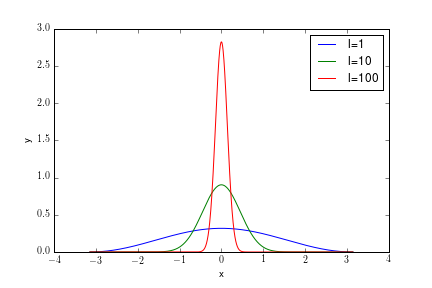
\includegraphics[width=0.40\textwidth]{figs/hk.png}}
\end{center}
\caption{\label{fig:hl} The function $h_\ell(x)$ for increasingly large values of $\ell$.}
\end{figure}

\noindent
To demonstrate the completeness of sines and cosines\footnote{This proof taken from http://web.mit.edu/jorloff/www/18.03-esg/notes/fourier-complete.pdf} we construct a peculiar but useful set of functions defined for $\ell=1,2,3,...$:
\begin{displaymath}
h_\ell(x) = c_\ell \left(\frac{1 + \cos(x)}{2}\right)^\ell
\end{displaymath}
We chose each factor $c_\ell$ such that:
\begin{displaymath}
\int_{-\pi}^{\pi} h_\ell(x) = 1
\end{displaymath}
The shape of $h_\ell$ is shown in Fig.~\ref{fig:hl}.  As $\ell$ increases, $h_\ell$ becomes more and more narrow at $x=0$, while the normalization is as in Equation~\ref{eqn:norm}.  It looks more and more like the delta function:
\begin{displaymath}
\lim_{\ell \to \infty} h_\ell(x) = \delta(x)
\end{displaymath}
It has one other important feature:  $h_\ell(x)$ is simply a sum of cosines of $nx$ with coefficients that don't depend on $x$.  To see how this can be, note that we can always turn a product of cosines into a sum via the trigonometric identity:
\begin{displaymath}
\cos \alpha \cos \beta = \frac{1}{2} \{\cos(\alpha - \beta) + \cos(\alpha + \beta)\}.
\end{displaymath}
So, for instance, we can write:
\begin{eqnarray*}
h_2(x) &=& \frac{c_2}{4} + \frac{c_2\cos(x)}{2}+\frac{c_2\cos^2(x)}{4} \\
           &=& \frac{c_2}{4} + \frac{c_2\cos(x)}{2}+\frac{c_2\cos(2x)}{8}
\end{eqnarray*}
This property implies that the function $h_\ell(x-a)$ for some constant $a$ is simply a sum of {\em both} sines and cosines of $nx$ with coefficients that don't depend on $x$, as:
\begin{displaymath}
\cos(nx-na) = \cos(nx)\cos(na) + \sin(nx)\sin(na).
\end{displaymath}

With this technology in hand we are ready to demonstrate the completeness of the sines and cosines.   
For simplicity, it suffices to consider only functions with period $L=2\pi$ (i.e. $k_n=n$).  The general case can then be inferred by transformation of coordinates.  Consider a real function $f(x)$ which is periodic for $L=2\pi$.  For now just define the function $F(x)$ to be the infinite series:
\begin{eqnarray}
F(x) \equiv a_0 + \sum_{n=1}^{\infty}  \left\{ a_n \, \cos(n x ) + b_n \, \sin(n x ) \right\}.
\end{eqnarray}
This is the compact form of the Fourier Series for this special case $L=2\pi$, so $k_n = n$.
We assume the coefficients are determined in the usual way:
\begin{eqnarray*}
a_n &=& \frac{2}{L} \int_{-\frac{L}{2}}^{\frac{L}{2}} 
f(x) \cos(n x) \, dx  \\
b_n &=& \frac{2}{L} \int_{-\frac{L}{2}}^{\frac{L}{2}} 
f(x) \sin(n x) \, dx.
\end{eqnarray*}
We need to show that $F(x) = f(x)$, or 
\begin{displaymath}
g(x) = F(x) - f(x) = 0
\end{displaymath}
The proof hinges on the fact that $F(x)$ and $f(x)$ have the same Fourier coefficients, so that:
\begin{eqnarray*}
\int_{-\pi}^{\pi} g(x) \sin(nx) dx &=& \int_{-\pi}^{\pi} F(x) \sin(nx) dx -  \int_{-\pi}^{\pi} f(x) \sin(nx) dx \\
&=& b_n - b_n \\
&=& 0 \\
\int_{-\pi}^{\pi} g(x) \cos(nx) dx &=& \int_{-\pi}^{\pi} F(x) \cos(nx) dx -  \int_{-\pi}^{\pi} f(x) \cos(nx) dx \\
&=& a_n - a_n \\
&=& 0 
\end{eqnarray*}
This shows that the integral of $g(x)$ times any sine or cosine is zero.  But our special function $h_\ell(x-a)$ function is just a sum of sines and cosines of $nx$ for any value of $a$.  This means that:
\begin{eqnarray*}
\int_{-\pi}^{\pi} h_\ell(x-a) g(x) dx &=& 0 \\
\end{eqnarray*}
If we take the limit as $\ell \to \infty$, we obtain:
\begin{eqnarray*}
\int_{-\pi}^{\pi} \delta(x-a) g(x) dx &=& 0 \\
g(a) &=& 0 \\
\end{eqnarray*}
Since this is true for any value of $a$, we have $g(x) = 0$ and so $F(x) = f(x)$.

\subsection{The orthogonality and completeness of the complex exponential function}

The first thing we need to show is that:
\begin{equation} \label{eqn:delta}
\frac{1}{2\pi} \int_{-\infty}^{\infty} \exp(ikx) \, dk = \delta(x)
\end{equation}
To see this we first calculate:
\begin{eqnarray*} \label{eqn:delta}
\frac{1}{2\pi} \int_{-a}^{a} \exp(ikx) \, dk &=& \frac{1}{2\pi} \, \frac{\exp(iax)-\exp(-iax)}{ix}\\
&=& \frac{1}{\pi} \, \frac{\sin(ax)}{x} \\
&=& \frac{a}{\pi} \, {\rm sinc}(ax)
\end{eqnarray*}
An integration shows that:
\begin{eqnarray}
\int_{-\infty}^{\infty} \frac{a}{\pi} \, {\rm sinc}(ax) \, dx = 1
\end{eqnarray}
exactly as needed for Equation~\ref{eqn:norm}.

Fig.~\ref{fig:sinc} shows that this function peaks at zero and becomes more and more narrow for progressively larger values of $a$.  Since it has the correct normalization, we conclude that:
\begin{eqnarray*}
\frac{1}{2\pi} \int_{-\infty}^{\infty} \exp(ikx) \, dk &=& \lim_{a\to\infty} \frac{1}{2\pi} \int_{-a}^{a} \exp(ikx) \, dk \\
&=& \lim_{a\to\infty} \frac{a}{\pi} \, {\rm sinc}(ax) \\ 
&=& \delta(x)
\end{eqnarray*}

\begin{figure}[thb]
\begin{center}
{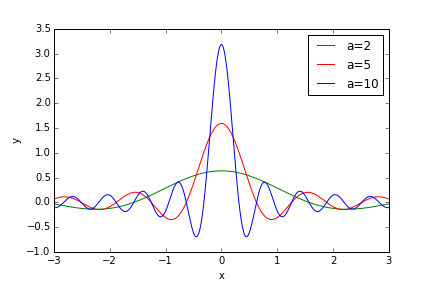
\includegraphics[width=0.40\textwidth]{figs/sinc.png}}
\end{center}
\caption{\label{fig:sinc} The function $a \, {\rm sinc}(ax)/\pi$ for progressively larger values of $a$.  As $a \to \infty$, this function approaches the delta function $\delta(x)$.}
\end{figure}

We are now fully equip to show that the complex exponential functions:
\begin{equation*}
e_k = \frac{1}{\sqrt{2\pi}} \exp(i k x)
\end{equation*}
are orthonormal.  Calculating the inner product
\begin{eqnarray*}
\braket{e_k, e_{k'}} &=& \int_{-\infty}^{\infty} \frac{1}{\sqrt{2 \pi}}  \exp(-ikx) \frac{1}{\sqrt{2 \pi}}  \exp(ik'x) \, dx \\
                               &=& \frac{1}{2 \pi} \int_{-\infty}^{\infty} \exp\{i(k'-k)x\} \, dx \\
                               &=& \delta(k-k')
\end{eqnarray*}
where we have used Equation~\ref{eqn:delta} but with the roles of $x$ and $k$ exchanged.
To prove completeness, we can now show that:
\begin{eqnarray*}
\Psi(x) &=& \int_{-\infty}^{\infty} \Psi(x') \, \delta(x-x') \, dx' \\
&=& \int_{-\infty}^{\infty} f(x') \left\{ \frac{1}{2 \pi} \int_{-\infty}^{+\infty} \exp\{ik(x-x')\} \, dk \right\} \, dx' \\
&=& \frac{1}{\sqrt{2 \pi}} \int_{-\infty}^{\infty} \left\{ \frac{1}{\sqrt{2 \pi}} \int_{-\infty}^{+\infty} f(x') \exp(-ikx') \, dx' \right\}  \exp(ikx) \, dk \\
&=& \frac{1}{\sqrt{2 \pi}} \int_{-\infty}^{\infty} \widetilde{\Psi}(k)  \exp(ikx) \, dk \\
\end{eqnarray*}
where:
\begin{eqnarray*}
\widetilde{\Psi}(k) &=& \frac{1}{\sqrt{2\pi}} \int_{-\infty}^{\infty} \Psi(x) \, \exp(-ikx) \, dx \\
\end{eqnarray*}





\end{document}




